\documentclass[conference]{IEEEtran}
\usepackage{enumitem}
\usepackage{graphicx}
\usepackage{url}
\usepackage{xcolor}
\usepackage{listings}
\usepackage[labelfont=bf,format=plain,font=small]{subcaption}
\usepackage[labelfont=bf,format=plain,font=small]{caption}
\usepackage{array}
\newcolumntype{L}{>{\arraybackslash}m{3cm}}
\usepackage{minted}
\newminted{sql}{mathescape, numbersep=5pt, frame=lines, framesep=2mm, fontsize=\footnotesize}
\usepackage{MnSymbol}
\def\prebreak{\raisebox{0ex}[0ex][0ex]{\ensuremath{\rhookswarrow}}}
\def\postbreak{\raisebox{0ex}[0ex][0ex]{\ensuremath{\hookrightarrow\space}}}
\def\lstbreak{\prebreak\newline\postbreak}
\lstdefinelanguage{pseudocode}{sensitive=false,morecomment=[l]{//},morestring=[b]",
                               morekeywords={if,else,while,continue,true}}
\lstset{breaklines=true,breakindent=5pt,
        postbreak=\postbreak,prebreak=\prebreak}

\newcommand{\todo}[1]{\textcolor{red}{TODO: #1}\PackageWarning{TODO:}{#1!}}


\begin{document}

% TODO playing with new ways of wording the title; the content we had was correct
% but I didn't feel great about the wording (and don't feel great about this either)
\title{Continuous Query-Based Syndication in the Cloud for Scalability and Availability}

\author{\IEEEauthorblockN{Gabriel Fierro}
\IEEEauthorblockA{gt.fierro@berkeley.edu}
\and
\IEEEauthorblockN{Erik Krogen}
\IEEEauthorblockA{erikkrogen@berkeley.edu}
}

\maketitle

\begin{abstract}
Applications in the Internet of Things exist at a confluence of semantically isolated networks over buildings, physical spaces, cloud services, smart appliances and mobile and wearable devices.
The utility of these applications is in their ability to capture capabilities of new families of smart, networked devices and integrate them with existing networks surrounding people, things and places.
We present a novel publish-subscribe mechanism --- continuous query-based syndication (CQBS) --- that allows subscribers to richly describe the set of resources they require and maintain a consistent view of relevant data sources even as they change over time.
We implement a highly available, distributed CQBS broker that uses a replicated coordinator to provide simple failover for embedded clients.
Through benchmarks, we demonstrate that the system maintains reasonable 95\textsuperscript{th} percentile latencies of under $10ms$ even under load.
\end{abstract}

\section{Introduction}

The context of the Internet of Things has seen an increase in both the number and capabilities of small, low-powered, constrained devices wanting to interact with each other and the outside world.
This has raised the question of how to conduct discovery and communication.
Publish-subscribe (pub-sub) is an attractive approach because it decouples publishers from subscribers in space (communication through a well-known broker helps deal with firewalls and NATs), and reduces load on popular publishers.

Ensembles of networked ``things'' interacting with dynamic applications require rich descriptive power to promote discovery across heterogeneous devices and services, which should be reflected in the syndication mechanism. They also require the ability to react to changes in the layout or configuration of devices, whether these changes are generated by the device or by a human administrator.
One of the characteristics that distinguishes the Internet of Things from prior collections of networked things is the higher number of devices in a space and the frequency with which those devices may enter or leave a space.
Applications or services may need to react to the entrance or exit of a device or user.
Discovery mechanisms that operate at discrete intervals---request-response or periodic advertisements---expect a delay proportional to the interval length.

There are two dominant ``flavors'' of pub-sub---topic-based and content-based---that traditionally identify tradeoffs between performance and expressiveness.
In topic-based pub-sub systems, messages are published to logical channels that may be in a flat or hierarchical namespace, and subscribers identify a name or ``glob'' that matches topics.
The benefits are that matching is typically fast and message overhead is small, but the expressive power of a ``topic'' is limited.
In content-based pub-sub, subscribers specify predicates, which act as filters for incoming messages for publishers.
While this scheme has richer descriptive power, it requires larger messages and computationally intensive brokers.

We propose an alternative pub-sub mechanism, continuous query-based syndication (CQBS), in which subscriptions are defined by SQL-style queries over device descriptions.
Device descriptions contain ``metadata'' defining properties of the device, e.g.\ location, units of measure, groupings, etc.\ that describe the context and configuration of the producer.
These queries are continuously evaluated to reflect the current configuration of all publishers, enabling subscribers to always receive messages relevant to their query even as the landscape of
publishers changes.

In this paper, we present the design and implementation of a distributed CQBS broker, a discovery service and message broker for service composition that uses \emph{continuous query-based syndication} to enable dynamic and contextually-aware applications and services for the Internet of Things.

Our design is motivated by a number of goals that we wish to achieve:
\begin{itemize}
\item High Availability: We wish to create a system that is resilient in the face of arbitrary machine failures.
\item Scalability: The system should be able to scale to large numbers of clients with reasonably high message rates.
\item Simple Clients: The code necessary for a client to interact with the system should be very simple, since we assume that they may be embedded devices with limited programming facilities.
\end{itemize}

We begin by outlining the core primitives of CQBS, \emph{streams}, which are virtual representations of specific sensor and actuator capabilities.
We then define the syndication model, which describes relationships between streams to create ad-hoc collections of capabilities needed for applications.
Syndication queries are expressed using SQL-like relations over stream descriptions and are continuously evaluated to maintain consistency with the environment.

%%% Local Variables:
%%% mode: latex
%%% TeX-master: "paper"
%%% End:
 % for later

\section{Related Work}

%TODO: do we define/justify the basic principles of pubsub anywhere here, e.g. decoupling between publishers and subscribers?

The CQBS distributed broker is most closely related to \emph{publish-subscribe} systems.
We examine each of the systems below along the primary design dimensions of the CQBS broker: richness of publisher descriptions, expressiveness of syndication model, client complexity and fault tolerance.

\begin{table*}
\caption{High-level comparison of features between systems}
\label{table:comparison}
\centering
\begin{tabular}{|l|c|c|c|c|c|}
\hline
\textbf{System Name} & \textbf{Publisher Descriptions} & \textbf{Syndication} & \textbf{Client Complexity} & \textbf{Client Failover} & \textbf{Fault Tolerant} \\
\hline \hline
redis~\cite{redis} & $N$ channels & List of channel names & Simple & None & Replicated cluster \\
MQTT~\cite{locke2010mq}\cite{hunkeler2008mqtt} & Hierarchical topics & Wildcard matching & Simple & None & None \\
XMPP~\cite{saint2011extensible} & Unique names & List of publishers & Complex & None & Federated Servers \\
Kafka~\cite{kreps2011kafka} & Hierarchical topics & Wildcard matching & Complex & Yes & Replicated broker cluster \\
SIENA~\cite{carzaniga2000achieving} & attribute-value pairs & SQL-like predicate & N/A & N/A & Replicated broker, flexible routing \\
\textbf{CQBS Broker} & attribute-value pairs & SQL-like predicate & Simple & Yes & Replicated brokers, coordinators \\
\hline
\end{tabular}
\end{table*}

\subsection{Topic-Based Publish-Subscribe}

Most publish-subscribe (``pubsub'') systems fall into one of two categories: topic-based and content based~\cite{eugster2003many}.
The most basic form of topic-based pubsub is a channel model, in which producers (data publishers) transmit data associated with some channel name to a broker; subscribers list the channels in which they are interested.
The benefits of this approach are its simplicity and speed---the ``hot path'' of a published message simply retrieves a list of subscribers---but there is limited expressive power because each publisher can only describe their data using a single dimension (the name of the channel)~\cite{redis}.
Because of these limitations, some modern pubsub systems use hierarchical topics with prefix and suffix matching using wildcards. The most popular of these are MQTT~\cite{locke2010mq}, Kafka~\cite{kreps2011kafka} and XMPP~\cite{saint2011extensible}.
%While our CQBS system is primarily a \emph{publish-subscribe} solution, its goals of providing
%resource discovery as well as data transfer means that we must also

%We examine each of the systems below along the primary design dimensions of
%the CQBS broker: richness of publisher descriptions, expressiveness of
%syndication model, client complexity and fault tolerance.

\textbf{MQTT} is a lightweight publish-subscribe protocol popular for its simpicity and extensible messages.
Producers of data in MQTT publish on hierarchical path-like topics such as \texttt{/apartment/gabe/livingroom/temperature}.
This construction of topics is best for grouping publishers together along a limited number of dimensions, but quickly becomes unwieldy as the dimensionality and sparsity of the descriptions increase.
For example, a temperature sensor could be described along the following dimensions:

\begin{itemize}
\item manufacturer and model number
\item city, campus, building, floor and  room number
\item orientation or position within a room
\item accuracy and precision of temperature sensor
\item method of temperature sensing (e.g. IR, thermopile)
\item who installed the temperature sensor and when it was installed
\item sample rate of the temperature sensor
\end{itemize}

To be effective, a topic-based system must determine the order and syntax of topics so that subscribers can know they are consuming the appropriate streams.
This is further complicated when considering other types of publishers which may include an entirely different set of descriptive tags.
MQTT syndication supports prefix matching on topics and limited forms of suffix matching.
To subscribe, applications specify explicit topics (\texttt{a/b/c/d}), one-level wildcards (\texttt{+/b/c/d, a/+/c/d, a/+/+/d, a/b/c/+}) and multi-level wildcards (\texttt{\#, a/\#, +/b/c/\#}).
While appropriate for basic subscriptions, this approach does not allow the expression of more complex predicates that contain ``and'', ``or'' or ``not'' relations: temperature sensors in Gabe's apartment, but not the ones in the kitchen or the bedroom.

MQTT supports three Quality-of-Service levels for message delivery: at most once, at least once, and exactly once.
Most client implementations simply address the first two, keeping complexity and code-size down; it is entirely feasible to implement a MQTT client on an embedded device, and there exists an adaptation of MQTT (MQTT-S~\cite{hunkeler2008mqtt}) for non-TCP/IP networks.
MQTT does not contain any explicit fault tolerance mechanisms: brokers may be distributed and ``bridged'' with the aid of an administrator, but failover logic is entirely implementation dependent.
In summary, MQTT is insufficient for our goals because hierarchical topics are fundamentally constraining in their structure and syndication.

\textbf{XMPP}~\cite{saint2011extensible}, or the Extensible Messaging and Presence Protocol, is an XML-based technology for instant messaging, video conferencing and more recently sensor communication (as seen in large, deployed systems such as Sensor Andrew~\cite{rowe2011sensor}).
Similar to channel-based systems, every entity (publisher or subscriber or broker) in a distribution of federated XMPP servers has some unique address from which it can send and receive messages.
There are attempts to provide a more expressive pubsub model on top of XMPP that allows for the discovery of services and subsequent subscription to relevant service providers~\cite{millard2010xep}.
These service descriptions can be extended to include arbitrary contextual data, which is a definite advantage over primitive address-based messaging.

The limitation of XMPP is in its size and complexity.
XMPP messages are XML-encoded and thus permit the expression of many different structures, but XML parsers are typically large and memory-intensive, rendering them inappropriate for embedded devices.
Additionally, XML tends towards large messages, which can result in fragmented messages in embedded networks that lower throughput and delivery rate.

\textbf{Apache Kafka}~\cite{kreps2011kafka} is a distributed messaging system designed for data pipelining in large, distributed, high-throughput applications.
Kafka is not designed for deployment scenarios that require rich descriptions of the array of available data services, so publisher and subscriber interactions are done via hierarchical topics and wildcard matching (very similar to MQTT).

Kafka, unlike MQTT and XMPP, is designed to be fault tolerant: all topics are replicated in a cluster of brokers, and failover is automatic.
To achieve the combination of fault tolerance and performance, Kafka clients must be carefully engineered, and are intended to be fuller applications rather than embedded devices.
Thus, while Kafka may be suitable for a data anaylsis pipeline in a datacenter, it does not meet our requirements for message delivery and reception at the ``edge'' of an IoT network.

\subsection{Content-Based Publish-Subscribe}

In content-based pubsub systems, publishers attach richer descriptions to messages, allowing subscribers to specify predicates that act as filters for which messages they receive.
While this scheme has richer descriptive power, routing on a per-message basis is computationally expensive (reducing routing efficiency) and can require larger messages from publishers.
% these will be fairly short

\textbf{SIENA}~\cite{carzaniga2000achieving}, the Scalable Internet Event Notification Architecture, aims to maximize the expressiveness of publishers and subscribers communicating in a wide-area network.
SIENA publishers send messages containing a set of \texttt{<type, name, value>} tuples, to which clients can subscribe using SQL-like filter expressions.
This approach, designed to provide discovery of relevant data in a large amount of heterogeneous messages, allows publishers to express richer metadata than would be feasible using a topic-based scheme.
It also allows subscribers to more precisely define the data they need.
For example, this could easily capture the proposed descriptive elements of the temperature sensor described above and allow a subscriber to filter on any combination of those attributes.

SIENA is fully distributed, using a tree overlay for routing and a special ``merging'' mechanism for pruning unnecessary delivery of messages to subtrees.
The disadvantages of SIENA mirror those of other content-based systems: carrying a full description of a publisher with every message reduces the bytes available for application data in embedded, constrained networks typical of the IoT.

\textbf{JMS}~\cite{hapner2002java}, the Java Message Service, is a distributed messaging service for connecting distributed application components.
Publishers send messages with headers containing standardized key-value pairs, but also contain lists of user-defined key-value properties.
Like SIENA, JMS clients subscribe with SQL-like expressions that express constraints on the set of publisher properties.
One difference between JMS and other systems is its default setting of exactly-once delivery, which complicates client logic and raises the network overhead of sending or receiving a message.

Distribution and fault-tolerance in JMS is possible, but requires specific configuration of which topics are distributed and among which servers they are distributed.
The focus of JMS is on enterprise-type applications that are in need of a messaging system that can adapt to its needs, but does not need to do so dynamically.

%\textbf{Elvin}

\subsection{Other Systems}

\textbf{Tuple Spaces} \todo{tuple spaces: t-spaces and linda}

\textbf{CORBA}~\cite{vinoski1997corba}, the Common Object Request Broker Architecture, is a data bus for communication amongst distributed objects that provides property- and name-based discovery and event notification.
Distributed object models (including DCOM~\cite{horstmann1997dcom}) share many features with content-based pubsub systems: similar to JMS, published messages contain key-value pairs in the header and body, and syndication is performed by subscribers specifying filters on those attributes.
CORBA itself is limited because it is not designed to be distributed, and has no failover or replication mechanisms.

%%% Local Variables:
%%% mode: latex
%%% TeX-master: "paper"
%%% End:
 % Gabe

\section{Continuous Query-Based Syndication}

Continuous Query-Based Syndication (CQBS) is a hybrid publish-subscribe pattern that provides the expressiveness of content-based systems while retaining the simplicity of topic-based systems.
The goal of CQBS is to provide a messaging system that can account for and adapt to the heterogeneity of data sources in the IoT.
CQBS endows embedded publishers to describe themselves using rich metadata, and provides subscribers to discover and subscribe to relevant data sources and maintain a consistent view of the context of those sources.

Here, we first establish the CQBS primitives --- streams and metadata --- before delving into how CQBS operates and what roles publishers and subscribers play.
We then describe the design and implementation of an individual broker (we defer the discussion of the full distributed system to Section~\ref{section:coordinator}.

\begin{figure}
\centering
\begin{lstlisting}[language=pseudocode,basicstyle=\small]
UUID = "dd9ef92e-140a-11e6-b352-1002b58053c7"
# register client
metadata = {
  UUID = UUID,
  Location/Room = "410",
  Location/Building = "Soda",
  Location/City = "Berkeley",
  Point/Type = "Sensor",
  Point/Measure = "Temperature"
  UnitofMeasure = "Fahrenheit",
  UnitofTime = "ms",
  Timezone = "America/Los_Angeles"
}
register_msg := msgpack.encode(metadata)
send_to_broker(register_msg)
while True:
    temp_val := read_sensor()
    msg := msgpack.encode({
            UUID = UUID,
            Value = temp_val
           })
    send_to_broker(msg)
    sleep(10)
\end{lstlisting}
\caption{Client registration and publishing pseudocode}
\label{fig:pseudoclient}
\end{figure}

\subsection{Streams and Metadata}

A stream is a virtual representation of a specific sensor or actuator channel (a ``capability'') that is indexed by a 16-byte universally unique identifier (UUID).
Each stream is described by \emph{metadata}, which is a bag of key-value pairs: keys are required to be string, but values may be any one-dimensional data type\footnote{In our implementation, values are restricted to strings: see Section~\ref{section:evaluation}.}.
Key-value pairs are most effective when drawn from some well-known ontology (such as Semantic Sensor Web~\cite{sheth2008semantic}), but our system places no restrictions on their content.
The association of metadata to a stream is done by the UUID; when a publisher creates a new stream, it registers that stream with the broker by sending a message containing the UUID and all of the metadata.
The broker (or the coordinator, in the distributed case) stores the mapping from stream UUID to metadata.
A publisher changes metadata by sending the ``diff'' of which keys and values have changed.
A given producer (data provider) can have as many streams as it wishes.
Each message contains at least the UUID of the originating stream, and can also contain any metadata changes, and of couse the published value itself, which can be any serializable object.

An example of metadata for a temperature sensor, and the basic client logic, can be found in Figure~\ref{fig:pseudoclient}.
In the initial registration message, along with the other metadata, the reporting process describes the thermostat as being in room 410 Soda.
If this changes, such as if the sensor were on a piece of smart clothing or furniture, the sensor attaches the metadata update \lstinline[language=SQL,basicstyle=\ttfamily]{Location/Room = "415"} to any outgoing message, where it is handled by the broker (described in the following section).
A discussion of client complexity can be found in Section~\ref{section:evaluation}.

This is a departure from the approach of content-based pubsub systems, where although the producer may possess some unique identifier, it transmits any associated ``content'' (metadata) in every message.
This verbose design choice may be appropriate for distributed sytems in which a publisher is a larger application that produces many different types of data, but when the data per-producer is relatively static (temperature sensors will always report temperature data), this flexibility is unneeded.
It becomes more efficient to essentially ``cache'' the metadata of a publisher in a central location where it can be used for syndication.

The simple structure of a stream (essentially a set of special key-value pairs) means a stream can be well represented in nearly any application protocol.
We choose MsgPack, a lean, typed binary serialization format that is simple enough to be encoded/decoded on embedded devices with limited code space.

%\subsection{Clients}

%Clients are distributed, continuously running processes that are producers and consumers of streams and updates to metadata.
%The streams produced by clients represent the set of sensors, actuators and capabilities available to be discovered, consumed and used.

% \emph{message} is the unit of communication in all interactions between
%clients and the broker. Messages sent from clients are either a query string
%for initiating a subscription or one-off response, or a structured packet
%containing the UUID of some stream and optionally an array of readings and/or a
%set of metadata updates. Examples of when metadata updates occur include when a
%device is registered (i.e.  sending the initial configuration), when a device
%changes location, or when a equipment attached to a device is changed such as
%installing an occupancy-driven switch for a lighting system.  Messages sent by
%the broker consist of forwarded client messages and ``diffs'' that convey
%changes in the set of streams matching a client's query.
%Figure~\ref{fig:messages} contains an example exchange of messages for
%a continuous query.
%
%Upon startup, a client registers streams it produces by sending messages
%containing metadata describing each one (see Figure~\ref{fig:message}). This makes
%the stream discoverable by and visible to other clients. Reporting data is
%straightforward: clients simply send messages with a stream's identifier and
%latest timestamped readings to the broker (the \texttt{UUID} and
%\texttt{Readings} fields). The broker forwards these readings to any subscribed
%clients as it receives them.
%
%In addition to producing streams, clients can also consume streams by
%expressing subscriptions to the broker in the form of SQL-like queries (see
%Section~\ref{section:syndication}). These queries are how clients perform
%discovery, receive timeseries data, and receive actuation requests.
%In dynamic environments typical of the Internet of Things, the results of
%these queries can become stale if they are executed only once. The broker
%continuously evaluates these queries to provide clients with a consistent view
%of their operating context.
%
%\subsection{Giles Architecture} \label{subsection:architecture}
%
%In this section, we present an overview of the six components of
%the Giles architecture.  These components handle incoming messages and queries
%for archival and delivery, and maintain consistent routes for query-based
%syndication.  This architecture is illustrated in
%Figure~\ref{fig:architecture}.
%
%\textbf{Protocol Plugin}: Protocol plugins do the work of translating messages
%between an application protocol and canonical message form. For
%simple request-response cases, the plugin translates the request, relays
%the message to the Giles API, then converts the result back to the original
%application protocol format and responds to the client. For the streaming
%functionality required by query-based syndication, the plugin maintains the
%connection to each client, and provides a handler to the Giles API that is
%called whenever an event is to be sent to an associated client.
%
%\textbf{API}: protocol plugins interface express how an incoming
%message should be interpreted. In terms of incoming data, Giles only deals with
%queries and messages (updates on streams involving metadata and/or new
%timeseries data), but can process them differently depending on the context.
%The API hands the incoming data to the correct pipeline.
%
%
%\textbf{Authorization Manager}: Giles enforces read/write permissions on a
%stream by stream basis. Considering the large numbers of devices and contexts
%predicted in the Internet of Things, it is important that
%administration of the system needs to scale, not just the system itself. Giles
%uses group-based permissions, rather than individual permissions, to avoid
%micromanagement of permissions surrounding increasing numbers of applications and users. All individual
%interactions with Giles carry an \emph{ephemeral key} which has an expiry and
%can be revoked; this key maps onto a set of roles. For each incoming
%interaction, the authorization manager does the work of evaluating the key's
%associated roles with the streams involved in the interaction, and adjusts the
%result set appropriately.
%
%\textbf{Broker}: While protocol plugins handle the network element of
%publishing and subscribing, the broker component provides routing
%between publishers and subscribers. This is done by maintaining mappings between clients, their associated
%queries, and the streams associated with those queries. These mappings are kept
%consistent in-band with the rest of the system, as discussed in
%Section~\ref{subsection:eventdriven} and seen in Figure~\ref{fig:evaluatequery}.
%
%\textbf{Query Processor}: The query processor parses all incoming queries and
%uses the outputted abstract syntax tree (AST) to adjust broker data structures
%(detailed in Figure~\ref{fig:evaluatequery}). This component also handles
%communication to and from the metadata and timeseries databases, and
%reevaluates subscription queries on behalf of the broker.
%
%\textbf{Timeseries Database}: Giles' role as a broker makes it a logical
%location to do archival of incoming data. Even in a distributed setting with
%multiple broker instances, Giles' visibility into all routed data means that
%archival can be performed without explicit action by clients. This is in
%contrast to other service composition systems (e.g. AllJoyn~\cite{alljoyn},
%SDS~\cite{czerwinski1999architecture},
%Jini~\cite{gupta2002jini}\cite{rigole2002using}\cite{waldo1999jini}) that
%perform archival as a secondary feature. All participants in such a system must
%duplicate all data to be archived and communicate that directly with an
%archival service. In Giles, all data and interactions are archived
%automatically and can be queried. Giles stores timeseries data in a dedicated
%timeseries store that is updated dynamically as clients report.
%
%\textbf{Metadata Database}: The Giles metadata model is simple enough to not
%place unusual requirements on the choice of a backend database.  Streams are
%wholly defined by their UUID and metadata, so the database only needs to store
%associations of UUID to metadata, and provide query facilities for retrieving
%metadata for a given UUID and retrieving all UUIDs whose keys fulfill a
%SQL-like predicate.  Stream metadata changes over time, which may invalidate
%any attempted categorization of streams. This makes the application of a strict
%relational schema unwieldy for maintaining the association of UUID to metadata,
%and informs our decision to impose structure over metadata using client-defined
%queries.

\subsection{Query-Based Syndication}

A primary contribution of our distributed broker architecture is its continuous, query-based syndication.
Queries are structured, SQL-like statements that define sets of constraints over stream metadata to express ad-hoc relationships between streams.
Query-based syndication is the use of these queries to define the forwarding routes from publishers to subscribers.
When an application sends a syndication query to the broker, that query is evaluated by the broker into a set of matching streams.
The broker constructs forwarding paths for those streams to the subscriber; whenever those streams send a message to the broker, it forwards that message to the relevant subscribers.

The resolution of queries to routes is \emph{continuous}; the broker reevaluates syndication queries as stream metadata evolves, and informs clients of changes in the set of the streams to which they are subscribed before adjusting the forwarding paths.
These changes happen on any metadata event: stream registration, stream deletion and metadata updates on streams.

\begin{table}
\caption{Supported key-value operations for the CQBS syndication query language}
\label{table:operations}
\centering
\begin{tabular}{|l|L|L|}
\hline
\textbf{Operator} & \textbf{Description} & \textbf{Example} \\
\hline \hline
\texttt{=} & Compare value equality & \texttt{Location/Room = 410} \\
\hline
\texttt{like} & Perl-style regex & \texttt{Manufacturer like "Dent\..*"} \\
\hline
\texttt{has} & Checks if the stream has the tag & \texttt{has Location/Building} \\
\hline
\texttt{and} & Logical AND of two subqueries & \\
\hline
\texttt{or} & Logical OR of two subqueries & \\
\hline
\texttt{not} & Inverts a clause & \\
\hline
\end{tabular}
\end{table}

\begin{figure*}[t]
\centering
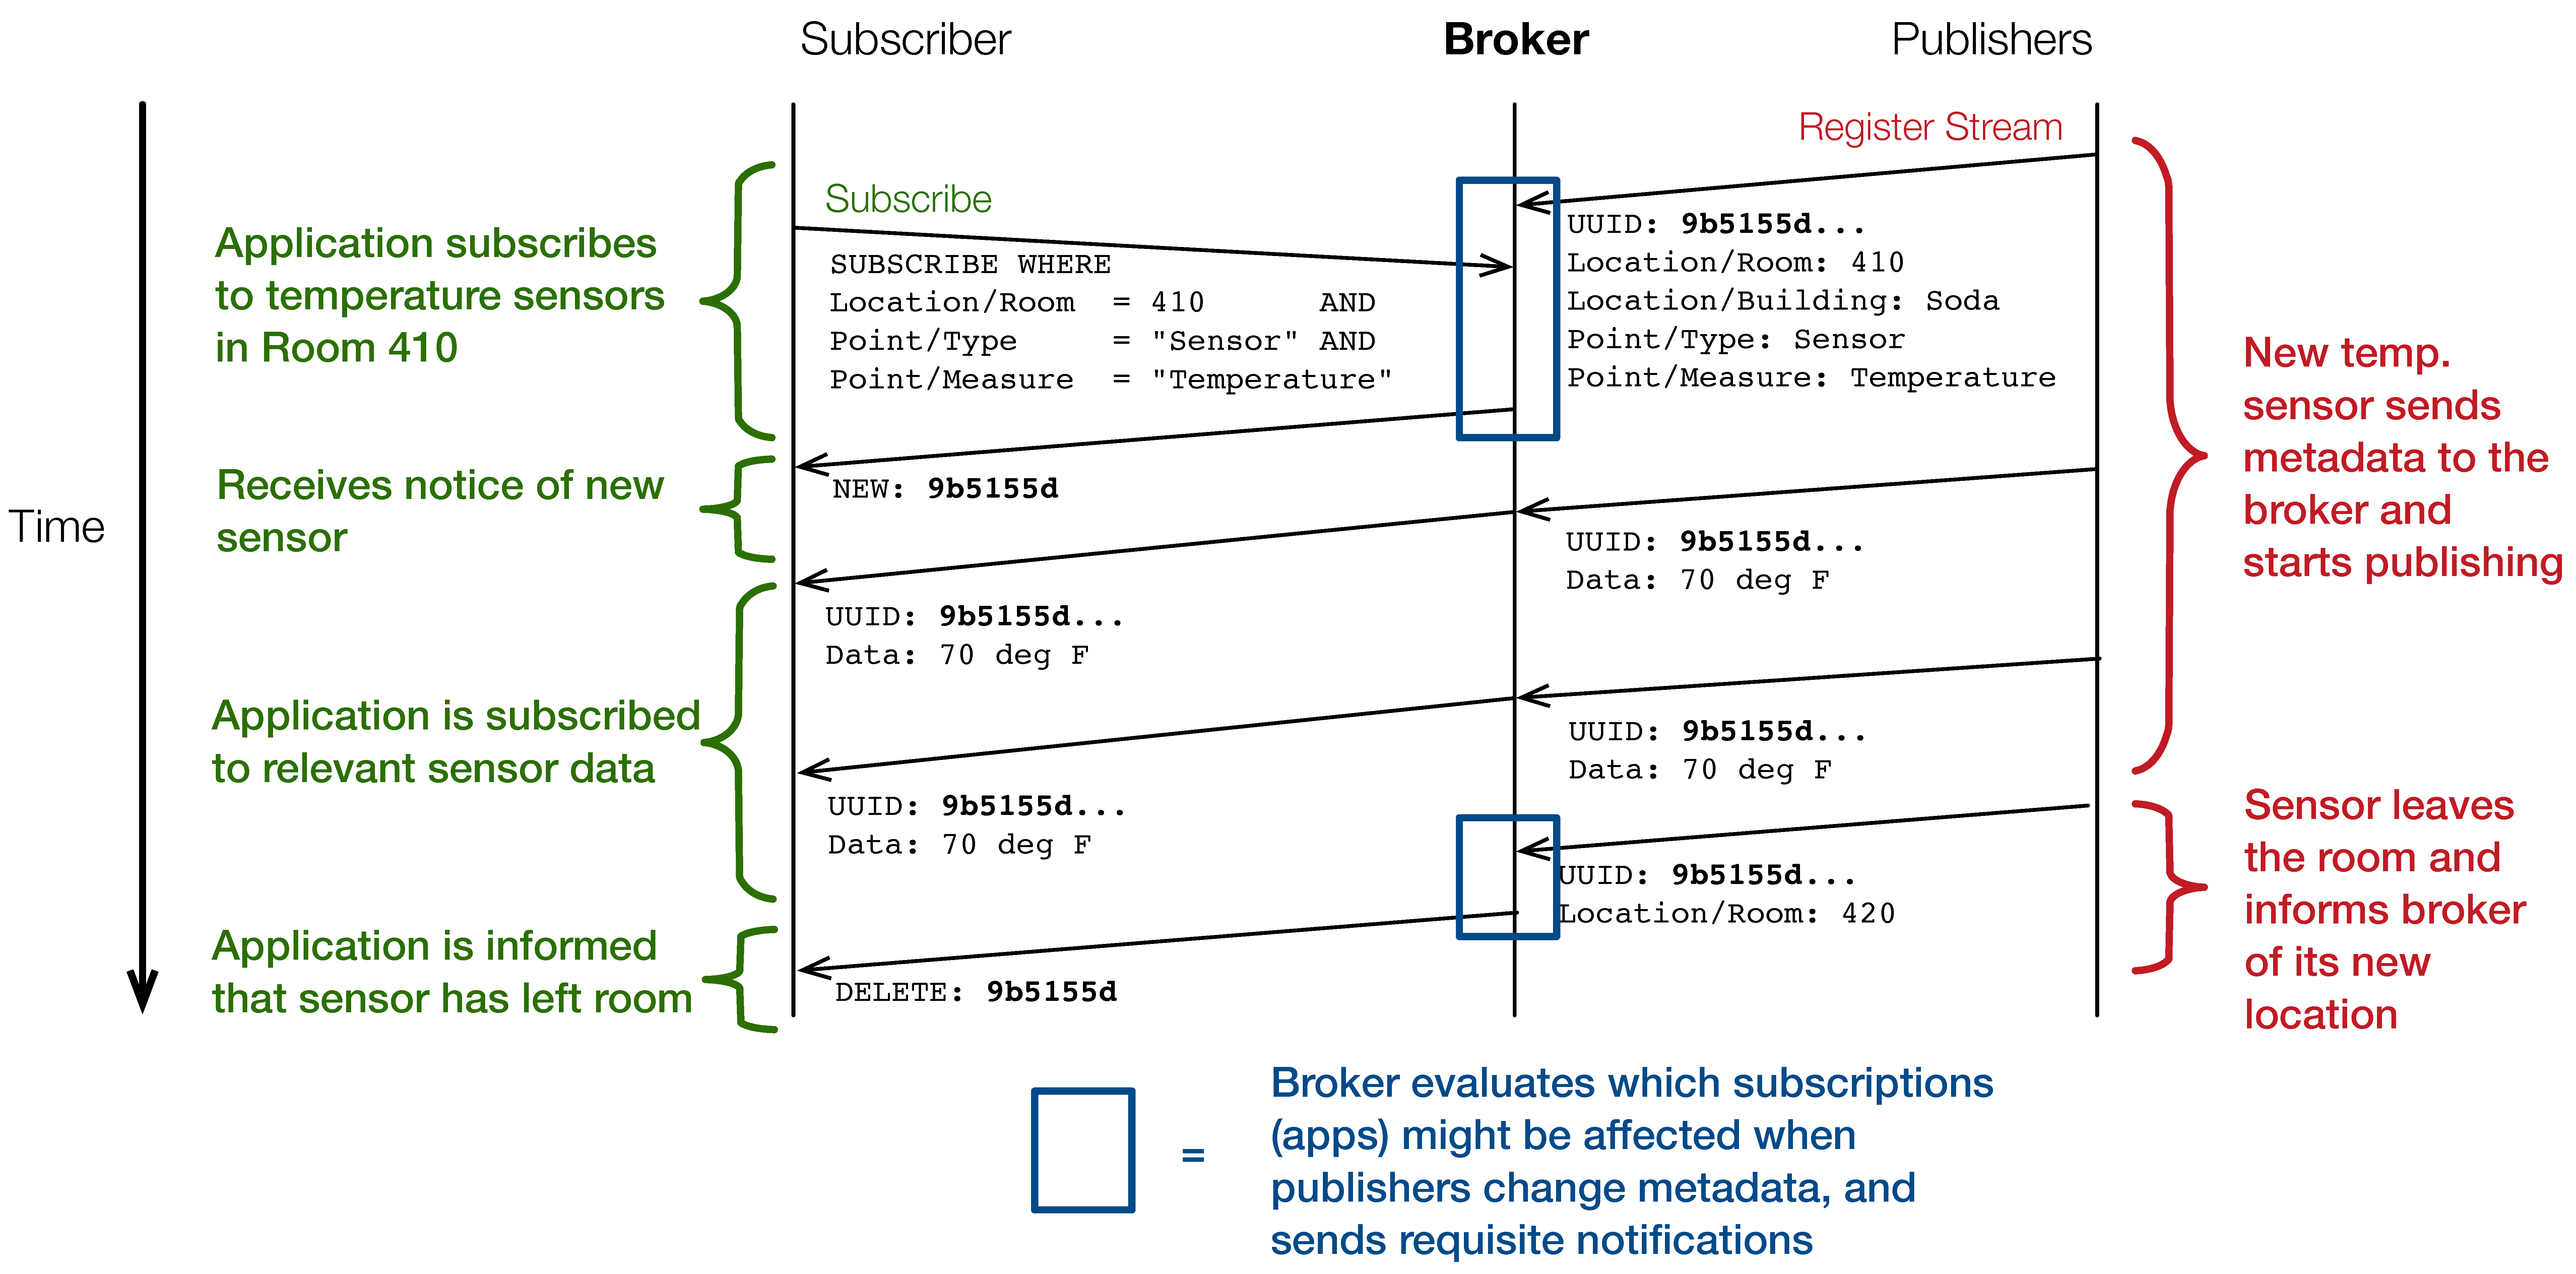
\includegraphics[width=.8\linewidth]{figs/messages.pdf}
\caption{The network traffic for a continuous query for discovering all temperature sensors in room 410 (ommitted
for brevity are additional constrains for building, units, etc). As new streams are registered, or their metadata
changes to no longer fit the discovery constraints, the client is updated in real-time.}
\label{fig:messages}
\end{figure*}


Queries are simple strings similar to the "where" clause of a SQL query. Table~\ref{table:operations} contains the set of available operations over keys and values.

For example, a hypothetical daylighting application wants to adjust the brightness of lights corresponding to how much natural light is entering a room.
It subscribes to the output of all dimmable lights in room 410 as well as all illumination sensors.
There are two subscriptions:

\begin{minipage}{\linewidth}
\begin{sqlcode}
-- dimmable lights
Room = 410 AND System = "Lighting"
AND has Actuator/Brightness
-- illumination sensors
Room = 410 AND Point/Type = "Sensor"
AND Point/Measure = "Illumination"
\end{sqlcode}
\end{minipage}
\vspace{0.3cm}

Figure~\ref{fig:messages} illustrates a typical exchange of messsages.
First, a temperature sensor stream with UUID (starting with) \texttt{9b5155d} is registered as being in Room 410.
Then, an application enacts a subscription to all temperature sensors in 410 Soda.
The broker evaluates this query against its metadata store, and establishes forwarding paths for those streams.
The broker then informs the subscriber of the set of streams it is subscribed to.
As the sensor publishes, its messages are forwarded to the subscriber.
Finally, the sensor is moved to another room --- perhaps as part of a piece of smart clothing or furniture --- and informs the broker of the change in its metadata.
The broker sees that the \texttt{Location/Room} tag has changed, so it looks internally for all syndication queries that contain the \texttt{Location/Room} key.
The broker reevaluates each of these queries, informs the application of the change in the set of its subscribed streams, and then adjusts the forwarding paths.

\subsection{CQBS Broker Design}

Continuous queries are an extension of traditional request-response relational queries to capture changes in a query's result set over time.
All incoming queries are evaluated against the metadata database or returned from a cache.
After the initial results of the discovery query are returned, the broker will continue to deliver updates on the result set to the subscribed client.

The broker maintains several data structures that are updated on any metadata event -- such as registering streams, deleting streams or streams changing metadata -- to avoid needing to reevaluate all registered subscriptions on every single event.
The data structures provide fast lookup of all queries that involve a given metadata key, and store the mapping from a query to the set of the UUIDs for matched streams.

We decouple the metadata and query mechanism from the underlying database by implementing the query language using Go-yacc.
This grants the ability to inject functionality at intermediate levels of the parsing process.
For each submitted syndication query, the broker extracts the set of metadata keys to optimize the query reevaluation process, which involves two data structures.

The key-query table (the first data structure) maps metadata keys to the set of queries that involve them.
Queries are consistently hashed to avoid amplification of the lookup table by duplicate queries with reordered clause terms.
Any incoming metadata event will have its keys referenced against this lookup table, generating a set of queries that will need to be reevaluated after the incoming metadata changes are committed.
The second data structure, the query-UUID table, stores which streams have been resolved for each query.
It is updated whenever a query is evaluated, and simplifies identifying which streams have entered or left a result set for a given query upon a metadata event.

\subsection{Implementation}

The CQBS broker is implemented in Go~\cite{go}, a statically typed, garbage-collected language with language-level support for concurrency in the
form of multithreading as well as handling asynchronous operations.
The language contains several built-in concurrency primitives: goroutines (lightweight processes), channels (for message passing) and a \texttt{select} statement (which helps implement non-blocking operations).
For these reasons, the Go language is a natural fit for developing highly concurrent network systems.

Go channels, in both the buffered and unbuffered varieties, make relaying backpressure straightforward.
Using channels to convey incoming and outgoing data between pipelined components means that when a component is too loaded to respond to pending tasks, it simply does not dequeue new tasks from the incoming channel.
This forces upstream components to block in relaying their tasks to that component, and results in cascading backpressure extending to the client~\cite{welsh2001seda}.
It is important to note that this backpressure is only applied to publishers when they are sending faster than the broker can sustain, \emph{not} when a particular subscribed client is overloaded.

Having to manage queries against an underlying database during metadata changes introduces a number of blocking operations into the ``hot path'' of the broker.
Goroutines, combined with synchronization primitives such as \texttt{sync.WaitGroup}\footnote{\url{https://golang.org/pkg/sync/#WaitGroup}} from the Go standard library, are a natural way to dispatch multiple concurrent operations in parallel and wait for their completion.
Goroutines are scheduled by the Go runtime, and scale nicely over multiple cores.

The design and implementation of Go does pose several challenges for low-latency systems.
First among these is the garbage collector, which is non-generational and mark-and-sweep.
Concurrent garbage collection was introduced in Go 1.5, but heap allocations do noticeably contribute to increasing latency.
Because Go is garbage collected, a large numbers of heap allocations can incur high latencies during
operation.
Many protocol encoder/decoders in Go create many temporary objects, and Go's compile-time escape analysis unnecessarily promotes many stack allocations to heap allocations, as revealed
in \cite{goescape}.

Using typed formats such as MsgPack, CapnProto and Protobuf allows parsing code to ``plan-ahead'' for which types to use and how much space they will use.
JSON is particularly bad at this; because it is a character-based format, parsing it requires many intermediate buffers and lookaheads to determine the size and type of elements in a received message.
Using generated code for encoding/decoding can drastically reduce the number of allocations. We use the excellent \texttt{msgp} library\footnote{https://github.com/tinylib/msgp}, which reduced the allocations per message from roughly 20 to 3.

%Using the broker as an intermediary for all client communication means
%that clients need only implement a single application protocol while retaining
%the ability to ``talk'' to any other client by means of the broker. The broker
%handles all routing of messages, and its protocol plugins handle all necessary
%conversions to and from a client's established protocol. This also means that
%duty-cycled embedded clients can be discovered even if they are not active at
%the time of some inquiry; embedded clients can pull persisted data like
%actuation requests and updated discovery results from the broker upon waking.

%Continuous query-based syndication is made tractable by the coordination of the broker and query processor.
%The query processor keeps those bindings consistent with streams' changing metadata.

%The Giles broker reevalutes these syndication queries as the underlying streams change, ensuring that subscribed clients always have up-to-date information on the state of the system.

%%% Local Variables:
%%% mode: latex
%%% TeX-master: "paper.tex"
%%% End:


\section{System Design} \label{section:coordinator}

% TODO ETK make sure 'publisher', 'subscriber', 'client' have all been defined by this point
% TODO ETK if these goals are already outlined somewhere else then no need to put them here

Our design is motivated by a number of goals that we wish to achieve:
\begin{itemize}
\item High Availability: We wish to create a system that is resilient in the face of arbitrary machine failures.
\item Scalability: The system should be able to scale to large numbers of clients with reasonably high message rates.
\item Simple Clients: The code necessary for a client to interact with the system should be very simple, since we assume that they may be embedded devices with limited programming facilities.
\end{itemize}

\subsection{Overview}

\begin{figure*}[t]
\centering
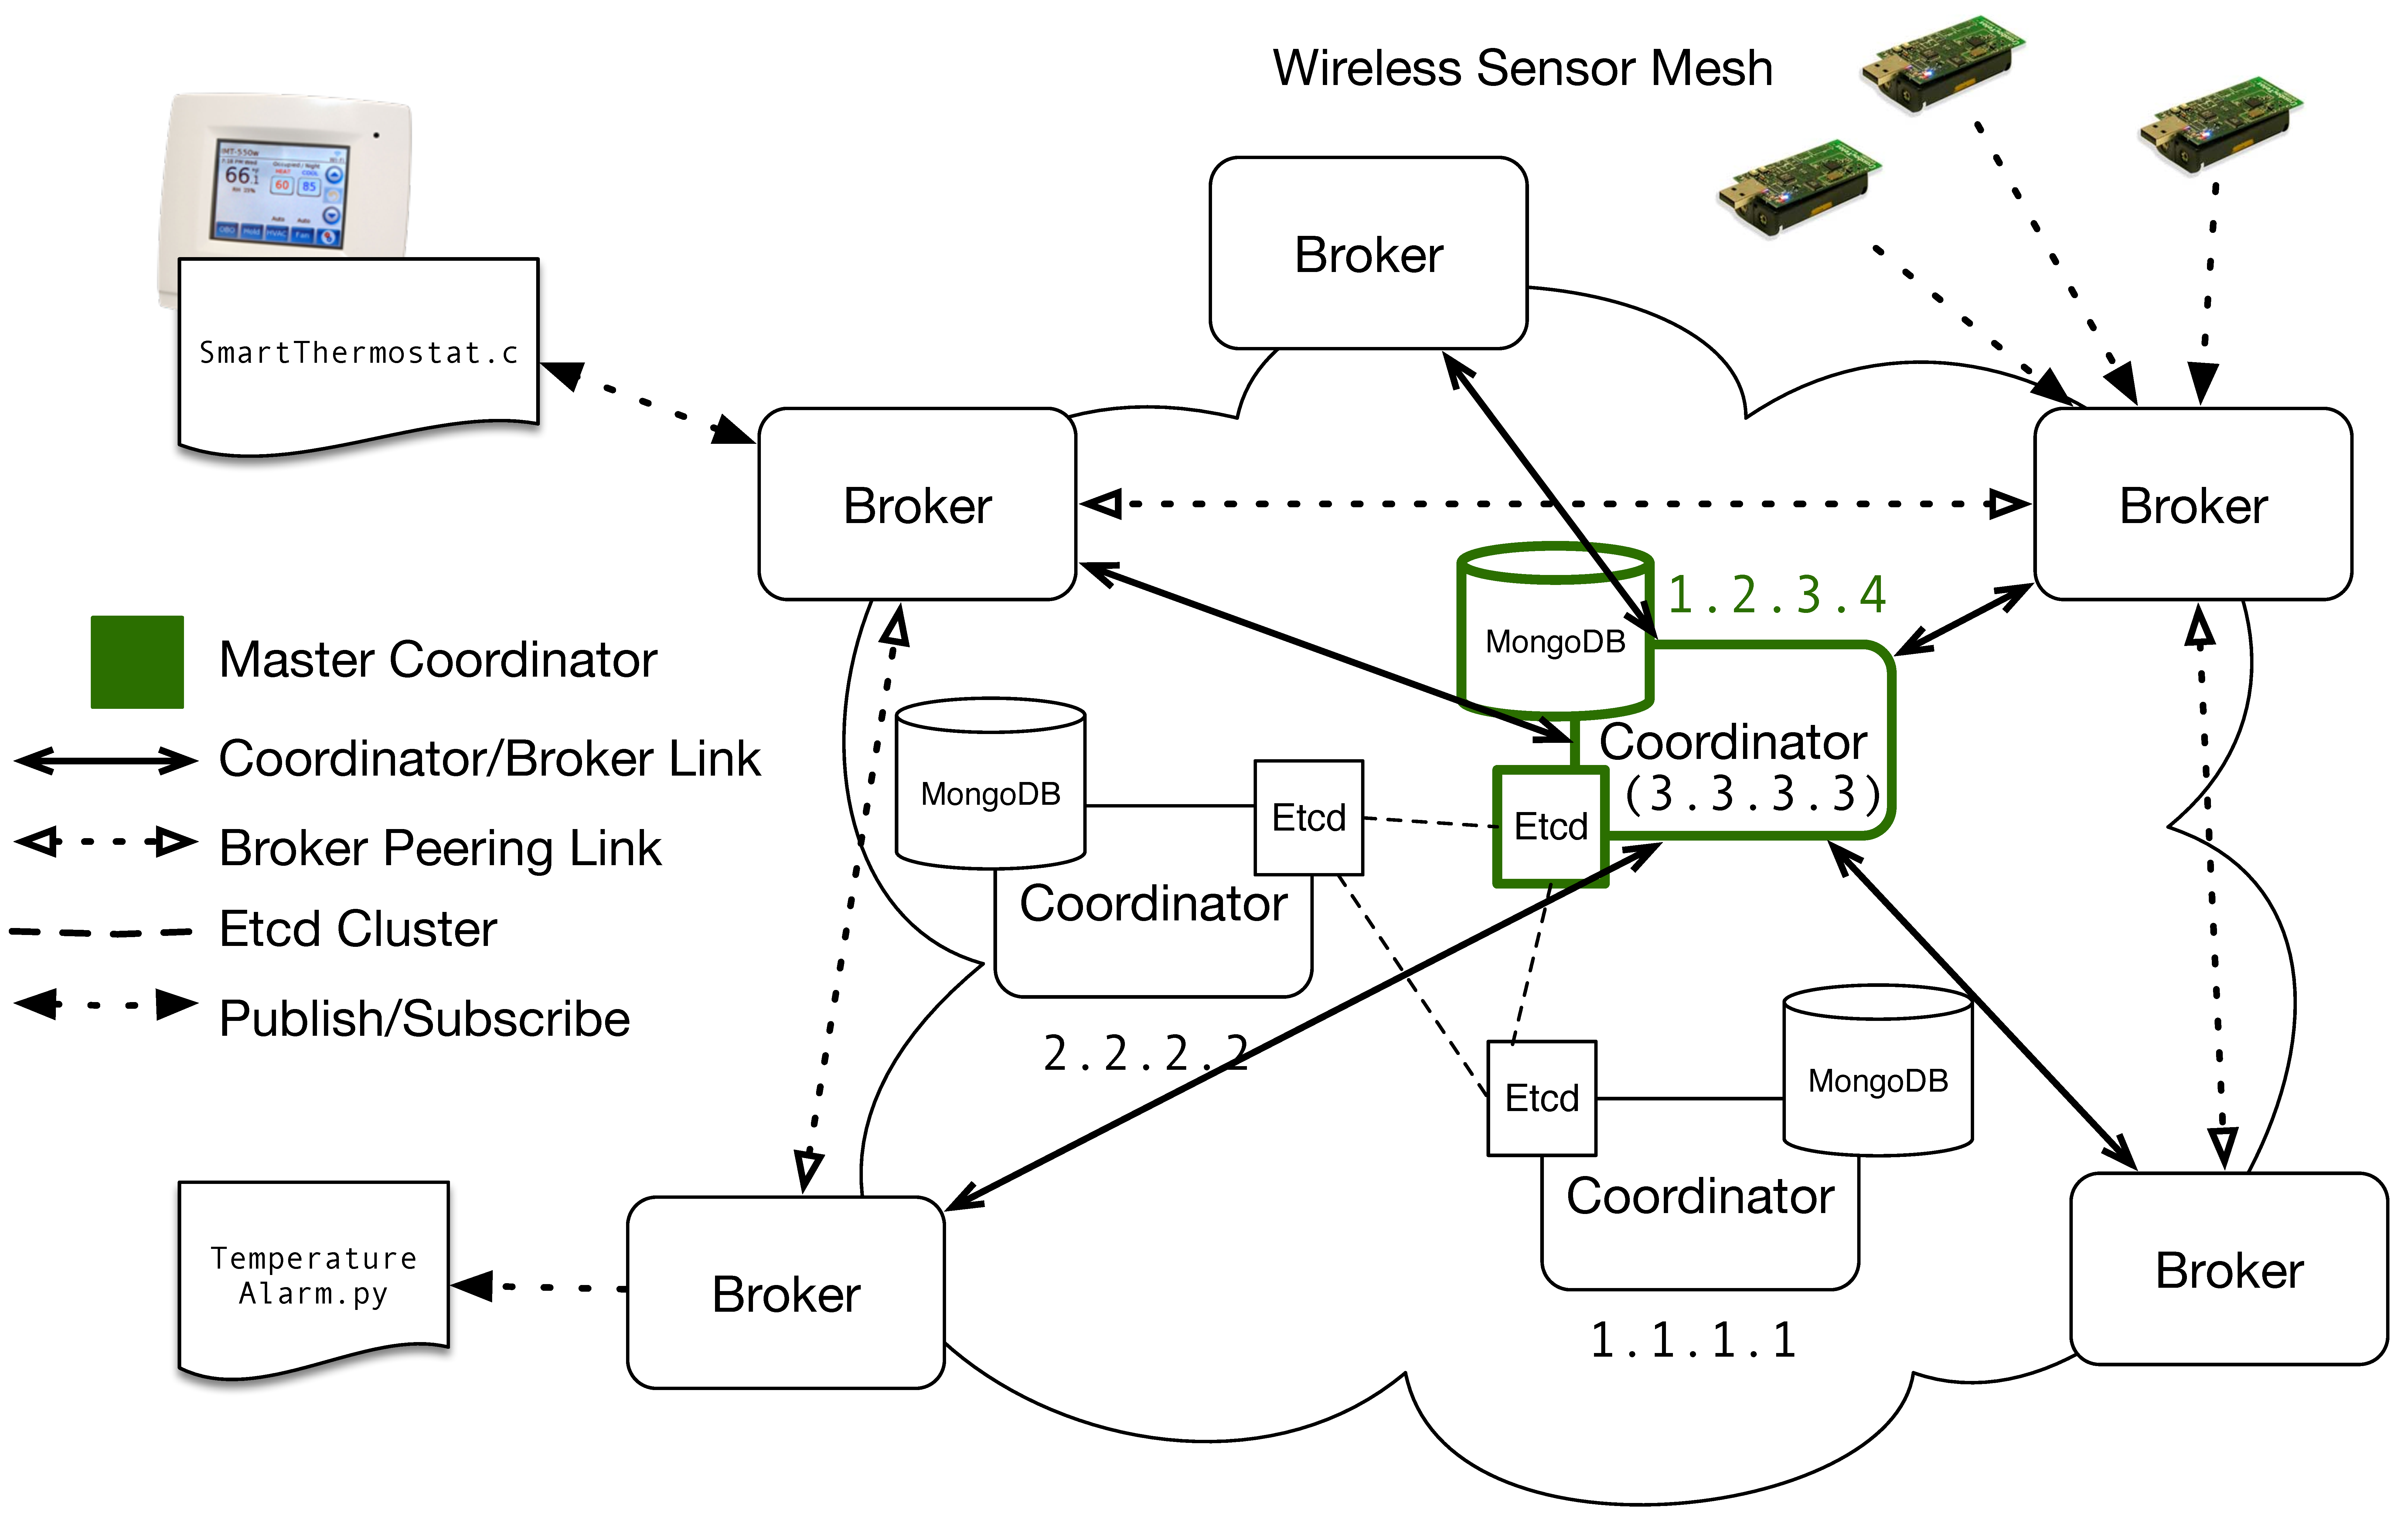
\includegraphics[width=6.5in]{figs/full_architecture.pdf}
\caption{Overview of the architecture of our brokerage system.
Numerous clients communicate to a set of decentralized brokers which create a forwarding network between themselves as instructed by the centralized coordinator nodes.}
\label{fig:architecture}
\end{figure*}

To meet these goals, we have developed an architecture which consists of two primary components: distributed brokers and centralized coordinators.
See Figure~\ref{fig:architecture} for an overview which will be described in more detail in this and the following sections.

The system contains one logically centralized coordinator; to all other entities in the system, the coordinator can be treated as a single machine.
In actuality, this logical coordinator consists of three independent nodes to improve fault tolerance; see Section~\ref{subsec:coordinator_fault_tolerance} for more detail.
This coordinator makes all of the decisions in the system, determining when a broker has failed, which brokers should forward which messages where, when changes occur to the set of publishers a subscriber is currently receiving messages from, which broker a client should contact if their broker fails, etc.
It then distributes these decisions to the brokers, which take appropriate action.
To do this the coordinator stores the current state of all brokers in the system, as well as information about all of the clients that are known to the system, i.e.\ what broker they are attached to, what query they are interested in (for subscribers), and what their current metadata is (for publishers).
Publisher metadata is stored in a local instance of MongoDB\footnote{\url{https://www.mongodb.com/}} which is used for executing queries.

Brokers are numerous and may reside anywhere; for example, a deployment may consist of a broker located in each building which contains client devices, or brokers may be run on cloud computing nodes.
Brokers are responsible for communicating with clients and for forwarding messages along routes as instructed by the coordinator.
Any changes to the set of clients connected to the broker, or to the metadata of a publisher connected to the broker, are communicated back to the coordinator for handling so that the coordinator always has an update-to-date view of the entire system state.

\subsection{Normal Operation}
\label{subsec:normal_operation}

In this section we describe the events which take place under normal operation, i.e.\ in the case that there are no failures within the system.

\textbf{A new subscriber enters the system.}
A subscriber contacts its local broker, Broker A, whose address can be hardcoded into the client or discovered through some network discovery protocol, e.g.\ % TODO Gabe can you help here
The subscriber submits a message to Broker A containing the query which defines which publishers' output it is subscribed to.
Broker A forwards the message along to the coordinator, which evaluates the query against the set of publisher metadata currently known to the system and replies to Broker A with the (possibly empty) set of relevant publishers.
If any relevant publishers are found, the coordinator will contact the broker at which they are located and instruct that broker to forward the publisher's messages to Broker A, which will in turn forward the messages to the subscriber.
We can see this, for example, in Figure~\ref{fig:architecture}: \texttt{SmartThermostat.c} is publishing to a broker which has a forwarding link established to another broker to which \texttt{TemperatureAlarm.py} is connected, establishing a publication route between \texttt{SmartThermostat.c} and \texttt{TemperatureAlarm.py}.

\textbf{A new publisher enters the system.}
A publisher contacts its local broker, Broker A, in the same manner as a new subscriber.
The publisher submits its initial set of key-value metadata pairs to Broker A, which forwards them to the coordinator.
The coordinator evaluates this new metadata against the set of currently active queries, notifies any subscribers whose queries apply to the new publisher, and constructs new forwarding routes from Broker A as in the previous case.

\textbf{A publisher submits new metadata.}
This process is essentially the same as adding a new publisher, except that in addition to possibly creating new forwarding links, some may need to be removed if the metadata changed in such a way that a publisher is no longer relevant to a subscriber's query.
Again, the coordinator will instruct Broker A about which brokers to create (and destroy) forwarding routes to.

\textbf{Clients leave the system.}
When subscribers and publishers leave the system, a similar process is followed; the coordinator is notified, and forwarding routes are created or destroyed as necessary.

\textbf{A publisher publishes a message.}
When a message does not contain any metadata changes, the coordinator is not involved in any part of the process.
The broker to which the publisher is connected simply broadcasts the message over all forwarding routes relevant to that publisher, and the recipient brokers will forward the message to the subscriber.

\subsection{Coordinator Fault-Tolerance}
\label{subsec:coordinator_fault_tolerance}

\begin{figure*}[t]
\centering
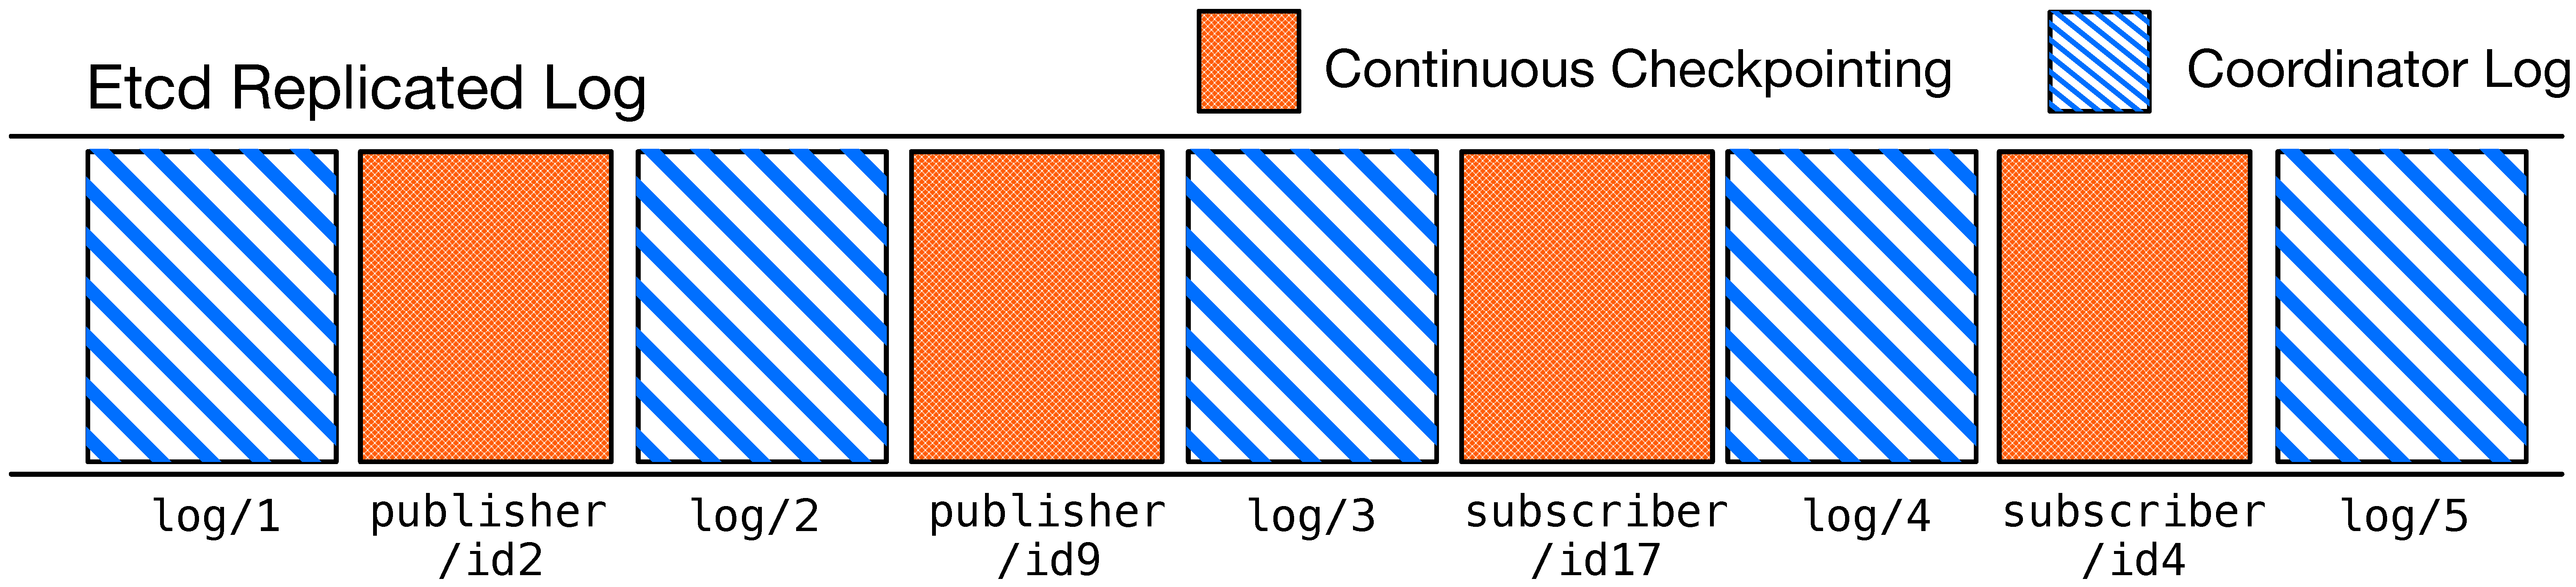
\includegraphics[width=.9\linewidth]{figs/logreplay.pdf}
\caption{Although they live in separate key spaces, the log and the continuous checkpointing are serialized via the Etcd log so that they can be leveraged for a consistent rebuild.}
\label{fig:logreplay}
\end{figure*}

To all other components of the system, including clients, the coordinator appears to be a single node which is resilient to failures; however, to construct a highly available system the coordinator must be able to handle at least one node failure.
To ensure that the coordinator will be resilient in the face of machine failure, we replicate its state across three independent nodes.
Each coordinator node runs an Etcd\footnote{\url{https://coreos.com/etcd/}} node, a reliable key-value store which internally uses the Raft distributed consensus protocol~\cite{ongaro2014} to provide strong consistency semantics among its members.
At any given time, one coordinator is designated as the leader; this is the only coordinator node which will accept messages from or send messages to brokers.
A single ``leader'' key is stored in Etcd; whichever coordinator was able to create this key via an atomic create-if-not-exists operation is considered the leader.
The key is marked with a time-to-live of a few seconds which is continually refreshed by the leader; if the leader fails to refresh its ownership of the key, the key will disappear, allowing another replica to become the new leader.

To make this cluster of machines with potential leadership changes appear to brokers and clients as a single machine, we maintain one external IP address at which the current leader can always be contacted (``1.2.3.4'' in Figure~\ref{fig:architecture}) in addition to the internal IP addresses which coordinators use to communicate with each other (``1.1.1.1'', ``2.2.2.2'', ``3.3.3.3'').
Various mechanisms can be used to ensure that this IP address always points to the correct coordinator; we run coordinator nodes on Amazon Web Services (AWS)~\footnote{\url{https://aws.amazon.com/}}, which provides an ``Elastic IP'' feature which allows for machine instances to request that an IP be reassigned to them.
Unfortunately the Elastic IP feature of AWS has delay of approximately 10--15 seconds (measured during our own experiments) before new requests are successfully routed to the correct host after the mapping has changed; this is a limitation of AWS and not fundamental to our protocol.

Every time a message is received from a broker, the leader logs the message to Etcd to make it durable before processing.
The replicas watch this log, continually applying log entries to their state as if they received the message from a broker.
This ensures that replicas are always very close to update-to-date with the state of the leader, lagging behind by only the latency of a write-read pair through Etcd (on the order of tens of milliseconds), making IP reassignment the only reason that coordinator failover is not extremely fast.
When the leader is finished processing a message, it sends an acknowledgment back to the originating broker.
If the broker does not receive an acknowledgment, it will resend the message.
So, if a leader writes a message to the log and crashes before finalizing its processing, the broker will eventually resend the message to the new leader, which ensures that the necessary operations are eventually completed.
Since messages are idempotent (e.g.\ attempting to create the same forwarding route twice has no effect the second time), it is acceptable for the new leader to redo some actions that the old leader carried out.

In addition to storing a log of inbound messages, the leader also stores the current state of each client and broker as a key-value pair within Etcd.
This is essentially a form of continuous checkpointing which enables a newly instantiated coordinator replica to quickly catch up to the state of the leader.
Rather than reading and executing the log from the beginning of time, a new replica can read the current state of the system via the client and broker keys up to some fixed point in time, then resume reading the log from that same point in time.
To maintain consistency between the continuous checkpoint and the log, we make use of the fact that Etcd internally maintains a sequential log of events (a consequence of using Raft).
Each modification to the Etcd store is marked with a revision number which indicates the order in which the modifications occurred.
By choosing some revision number and reading all client/broker state up to and including that revision, then reading all log entries after that revision, it is ensured that the replica switches from reading the checkpoint to reading the log in a consistent manner.
Note that this works even if the client or broker key was overwritten (i.e.\ if a change to the state occurred which was then written to Etcd) because Etcd stores versioned copies.

To clear old checkpoint versions and unnecessary log entries, the leader periodically performs garbage collection.
Replicas periodically write the sequence number of the last log entry they processed to a specific key in Etcd.
The leader periodically checks these values and instructs Etcd to delete entries which both replicas have already read, as well as instructing Etcd to perform a ``compaction'' up to this point, which removes old versions of keys which are no longer needed.

\subsection{Broker Fault-Tolerance}

In addition to being resilient to coordinator failures, we require that our system continue functioning and all clients continue to be able to participate in the face of a broker failure.
To this end, and with low client complexity in mind as a goal, we have designed a very simple fail-over protocol which allows the client to continue to operate on another broker during the period in which its local broker is not available.

In addition to being aware of its local broker as described in Section~\ref{subsec:normal_operation}, each client must know the external address of the coordinator.
First, a client attempts to contact its local broker, Broker A.
If the client is unable to do so, it sends a request to the coordinator, which will supply it with the address of some other broker B which can service its needs until Broker A is available again.
The client connects to Broker B and continues as usual.
When Broker A becomes available, the coordinator instructs Broker B to sever its connection to the client, which will then attempt to contact Broker A as usual. This can be summarized by the following pseudocode:

% TODO maybe could use some work
\begin{lstlisting}[language=pseudocode,basicstyle=\small]
while client_active:
  success := connect_to(local_broker_address)
  if success:
    // process ...
  else:
    broker_addr := connect_to_get_message(coordinator_address)
    success := connect_to(broker_addr)
    // process ...
\end{lstlisting}

\subsection{Design Discussion}

This design allows us to meet all of our goals.
We have high availability via fault tolerance for both broker and coordinator failures.
The necessary code for clients is very simple; publishers need to know how to send publication messages, subscribers need to know how to send query messages and receive publication messages and subscription difference messages (e.g.\ publisher A just became relevant to your query), and both need to know how to ask the coordinator for a fail-over broker.
We also have scalability in terms of number of messages that can be sent through the system by removing any coordination from the normal message forwarding path, which can be scaled arbitrarily with the number of brokers.

One aspect on which this design is lacking is that the coordinator is a bottleneck for changes to the state of the system (i.e.\ clients entering or leaving and publishers changing metadata).
We assume that in comparison to the rate of messages being sent in the system, changes to the set of connected clients and to the metadata associated with publishers is relatively slow, so we consider this design to be acceptable.
Part of the reason for choosing this design was its relative simplicity; we have considered two alternate designs which were considered and which we hope to evaluate as future work (see Section~\ref{subsec:alternate_designs})..

%%% Local Variables:
%%% mode: latex
%%% TeX-master: "paper"
%%% End:


\section{Evaluation} \label{section:evaluation}

Here we present the evaluation of a distributed CQBS broker.
All brokers and coordinators machines were chosen to emulate commodity hardware; for CQBS to be an effective solution, it must not rely on intractably large resources.
Hence, we chose to use the \texttt{t2.medium} AWS instance type with 2 vCPUs and 4 GB RAM, running Ubuntu 14.04.
As we will demonstrate below, the CQBS system is amenable to commodity systems because its performance is limited by the serialization of the etcd log, and not by memory, CPU, disk, or network bandwidth.

\subsection{Performance}

\begin{figure}[t]
\centering
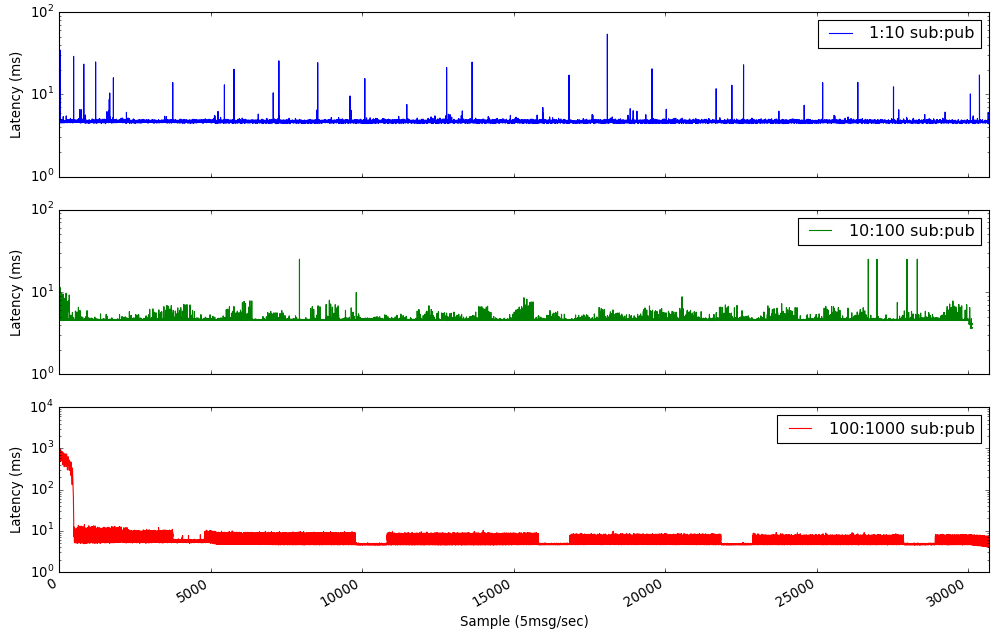
\includegraphics[width=\linewidth]{figs/singlenodelatency.png}
\caption{Microbenchmark: standalone CQBS broker forwarding latency with increasing concurrency}
\label{fig:singlenodelatency}
\end{figure}

First, we examine the latencies of the CQBS broker's forwarding mechanism in isolation -- without the communication overhead imposed by the fully replicated system.
We run a single broker on a \texttt{t2.medium} instance, backed by MongoDB.
Using a ratio of 10 publishers to one subscriber, we run three benchmarks with 1, 10 and 100 subscribers (with 10, 100 and 1,000 publishers accordingly).
Each publisher sends 5 messages per second; after the initial registration message (the high latencies at the beginning of each benchmark), each publisher sends only its stream UUID and an increasing counter as its value.
Each group of publishers/subscribers use entirely isolated sets of keys, so that they do not explicitly interfere with each other in the broker.
These three microbenchmarks are shown in Figure~\ref{fig:singlenodelatency}, and demonstrate that the latency is fairly consistent as the amount of concurrency scales.

The spikes in latency seen in the $N=1,10$ graphs are due to the pauses enacted by Go's garbage collection.
Fortunately, these do not affect the vast majority of requests.
For the $N=1,10$ cases, the mean latencies, 95\textsuperscript{th} percentile latencies and standard deviation are $4.67ms/4.85ms/0.55ms$ and $4.62ms/4.77ms/0.37ms$ respectively.
For the $N=100$ case, the garbage collection becomes more visible in the variability of response times, with mean, 95\textsuperscript{th} percentile and standard deviation latencies of $13.58ms/8.87ms/67.13ms$.
The troughs in the $N=100$ case are an odd phenomenon, most likely caused by garbage collection in the single Go process used to generate the 100 subscribers and 1000 publishers, generating approximately 5000 messages per second.

\subsection{Client Complexity}

\subsection{Fault Tolerance}


\section{Future Work}

\subsection{Comparative Evaluation}

While researching previous systems, we found many that purport to solve similar problems or had similar approaches (Section~\ref{section:relatedwork}); however, many of these systems are difficult to evaluate for at least one of the following reasons: they are an aging research system that no longer has an actively maintained codebase, the distributed nature was never fully explained or implemented, or most commonly, emulating the desired behavior to directly compare to our CQBS system involved an inordinate amount of implementation.
For these reasons, we decided to focus our evaluation on the behavior of our own system, and defer an explorative comparison to other systems for future work.

\subsection{Alternate Designs}
\label{subsec:alternate_designs}

\todo{this could probably be cleaned up a little}

Currently, a full Raft transaction is performed through Etcd on every change to the system state.
While this provided a relatively simple design with strong consistency guarantees, it incurs a rather high latency that does not parallelize due to the serial nature of Raft transactions.
One alternate method to explore would be to use Raft only for leader elections, and have the leader stream events directly to the other coordinators rather than submitting them to the Etcd log.
It may be possible to achieve higher throughput using, for example, a 2-phase commit protocol.

Currently, the full state of the system is stored only at the coordinator, which can become a scalability bottleneck.
We have considered one alternate design which is essentially the opposite of this, with the coordinator storing no system state beyond the set of connected brokers.
On inbound queries and metadata changes, a broker would broadcast to all other brokers, allowing them to evaluate the changes and set up new forwarding routes as necessary.
This is unfortunately expensive as it requires a broadcast, but it does away with the necessity for replication via Etcd since brokers can recreate the state of their system via information they receive when clients reconnect to them, which may be a desirable tradeoff.

Another option we considered that provides a tradeoff between our current design and the one described above would be to have each broker store only its own state, and have the coordinator store only some sort of heuristic data.
A broker would forward messages to the coordinator, which would not contain the full system state, but have enough information to narrow the possibly affected brokers to a smaller subset as opposed to having to broadcast to the entire system.
This could, perhaps, mean storing ranges of metadata values that publishers at brokers contain.
This pushes off the query processing effort onto the brokers and avoids full system broadcasts, making it scalable, but unfortunately still requires the coordinator to have a consistent view of the system to avoid the situation where the coordinator doesn't forward a message to a broker which it should have.
However, as this view of the system is only required for performance rather than correctness (since all messages could still be broadcast), it may prove to be a desirable point in the design space.

%%% Local Variables:
%%% mode: latex
%%% TeX-master: "paper"
%%% End:


\section{Conclusion}

This paper presents the design and implementation of a distributed broker that implements continuous query-based syndication over richly-defined streams.
The CQBS broker, which is implemented in Go, offers more expressive power while remaining tractable to implement on embedded, constrained clients typical of the Internet of Things.
CQBS strikes a middle ground between the fast but restricted descriptive power of topic-based pubsub systems and the rich descriptive power but heavyweight nature of content-based pubsub.
Above this, we demonstrate how the system can be made highly available using a logically-centralized replicated coordinator to maintain consistency between distributed brokers.


\bibliographystyle{IEEEtran}
\bibliography{IEEEabrv,references}

\end{document}



%%% Local Variables:
%%% mode: latex
%%% TeX-master: t
%%% End:
